\documentclass[a4paper,12pt]{article}

\title{Biology 30 IB \\ Populations}
\author{Jad Chehimi}

% document setup
\renewcommand{\familydefault}{\sfdefault}
\linespread{1.25}
\usepackage[margin=1in]{geometry}
\usepackage{setspace}
\usepackage{enumitem}
\setlist{nosep}
\usepackage{color,soul}
\setcounter{secnumdepth}{0}

% tools
\usepackage[hidelinks]{hyperref}
\usepackage{float}
%% images
\usepackage{graphicx}
\graphicspath{ {./images/} }
%% science
\usepackage{siunitx}
%% chemistry
%\usepackage[version=4]{mhchem}

\begin{document}
\maketitle

% temp
\begin{center}
\Huge
Unfinished!
\normalsize
\end{center}
% temp

\tableofcontents

\pagebreak

\begin{itemize}
    \item{Most species have thousands of genes}
    \item{More genes = more genetic diversity}
    \item{More alleles in said genes = more genetic variation}
    \item{Genetic diversity increases from sexual reproduction}
\end{itemize}

\section{Human Populations}
\subsection{Problems with Human Genes}
\begin{itemize}
    \item{Few offspring}
    \item{Observations take time}
    \item{Many traits affected by environment as well as genes}
\end{itemize}

\subsection{Population Sampling}
\begin{itemize}
    \item{Technique used to study human populations}
    \item{\textbf{Representative group} = group within population is selected, not entire population}
    \item{\textbf{Trends} or \textbf{Frequencies} = how often genes occur in the representative group}
    \item{\textbf{Gene pool}, aka. \textbf{genome} = all genes in a population}
    \item{\textbf{Fixed frequency} = only 1 allele for a gene, all organisms in population has gene}
\end{itemize}

\subsubsection{Frequency}
\begin{itemize}
    \item{\textbf{Genotype frequency} = proportion of a population with a particular genotype (expressed as a decimal)}
    \item{\textbf{Phenotype frequency} = proportion of a population with a particular phenotype (expressed as a decimal or \%)}
    \item{\textbf{Allele frequency} = rate of occurrence of a particular allele in a population with respect to a particular gene (expressed as a decimal)}
\end{itemize}

\section{Hardy Weinberg Principle}
\begin{itemize}
    \item{
            Populations have either a...
            \begin{itemize}
                \item{tendency to remain stable}
                \item{tendency toward variability}
            \end{itemize}
        }
    \item{\textbf{Genetic equilibrium} = if all other factors remain constant, the gene pool will have the \hl{same composition generation after generation}}
    \item{Population \hl{evolve} when \hl{equilibrium is upset}}
\end{itemize}

\subsection{Hardy Weinberg Equilibrium}\noindent

\begin{enumerate}
    \item{
            \Huge $$p + q = 1$$ \normalsize
            \begin{itemize}
                \item{\hl{Allele frequency}}
                \item{$p$ = frequency of dominant allele (e.g. A)}
                \item{$q$ = frequency of recessive allele (e.g. a)}
            \end{itemize}
        }
    \item{
            \Huge $$p^2 + 2pq + q^2 = 1$$ \normalsize
            \begin{itemize}
                \item{\hl{Genotypic frequency}}
                \item{Above formula, but for all heterozygote father and heterozygote mother crosses}
            \end{itemize}
        }
\end{enumerate}

\subsubsection{Tips}
\begin{itemize}
    \item{A = $p$, a = $q$}
    \item{AA = $p^2$, Aa \& Aa = $2pq$, aa = $q^2$}
    \item{Work with homozygous recessive individuals first \\ (only one possible genotype --- homozygous recessive)}
\end{itemize}

\subsection{Conditions of No Evolution}
Conditions under which no change will occur in a gene pool are...
\begin{itemize}
    \item{Large populations = changes in gene frequencies are not the result of random chance alone}
    \item{Random mating}
    \item{No mutations}
    \item{No migration = no immigration, no emmigration, no new genes enter or leave the population}
    \item{Equal viability (no disease), fertility, and mating ability of all genotypes (no selection advantage)}
\end{itemize}

\pagebreak

\subsection{(21.2) Conditions of Evolution} \noindent

The population gene pool is very unstable.

Conditions under which change will occur in a gene pool are...
\begin{itemize}
    \item{
            \textbf{Mutation}
            \begin{itemize}
                \item{Changes in the genetic makeup, either chromosome mutation or gene mutation}
                \item{Occurs during meiosis}
                \item{May be harmful in some parts and beneficial others \\ e.g. sickle cell anemia carriers (heterozygous) have malaria resistance}
            \end{itemize}
        }

    \item{
            \textbf{Migration} (aka. Gene Flow)
            \begin{itemize}
                \item{Movement of members of a species, into (immigration) or out of (emigation) a population}
                \item{\textbf{Immigration} = new genes are added to existing gene pool}
                \item{\textbf{Emigation} = genes are removed}
            \end{itemize}
        }
    \item{
            \textbf{Non-random Mating} (aka. Sexual Selection)
            \begin{itemize}
                \item{Choice of which males will mate with which females}
                \item{Choice often made by woman, based on physical or behavioral traits of mate}
                \item{\textbf{Sexual dimorphism} = difference between male and female phenotypes (e.g. mane, antlers)}
            \end{itemize}
        }
    \item{
            \textbf{Small Populations}
            \begin{itemize}
                \item{
                        \textbf{(Random) Genetic Drift}
                        \begin{itemize}
                            \item{Disruption of genetic equilibrium in small populations}
                            \item{If a unique allele does not mate, the allele is gone forever}
                        \end{itemize}
                    }
                \item{
                        \textbf{Founder Effect}
                        \begin{itemize}
                            \item{Few individuals of large population leave, forms new population}
                            \item{Allele frequencies will not be the same as former population}
                        \end{itemize}
                    }
                \item{
                        \textbf{Bottleneck Effect}
                        \begin{itemize}
                            \item{Severe environmental event, drastic reduction in population size}
                            \item{Allele frequencies very different than original population}
                        \end{itemize}
                    }
                \item{
                        \textbf{Natural Selection}
                        \begin{itemize}
                            \item{Only process that leads directly to evolution}
                            \item{Individuals with greater survival traits reproduce, passing on their favorable genes to the next generation}
                        \end{itemize}
                    }
            \end{itemize}
        }
\end{itemize}

\pagebreak

\section{Mitochondrial DNA \& Evolution}
\begin{itemize}
    \item{\textbf{mtDNA} = Mitochondrion contain their own genetic material}
    \item{Mitochondria and chloroplast were once individual organisms, but symbiotic relationship formed with cells}
    \item{Mutations in mtDNA = Parkinson's}
\end{itemize}

\section{Speciation}
\begin{itemize}
    \item{Process by which species originate}
    \item{
            \textbf{Species} = organisms that can...
            \begin{itemize}
                \item{\hl{interbreed}}
                \item{\hl{produce fertile offspring}}
            \end{itemize}
        }
\end{itemize}

\subsection{Geographic Isolation}
\begin{itemize}
    \item{Caused by \hl{physical obstacles/barriers}}
    \item{Gene flow between main population and isolated group ceases}
    \item{
            Eventually, new species; become so genetically different that they can \hl{no longer interbreed}, due to...
            \begin{itemize}
                \item{different adaptations}
                \item{different gene frequencies}
                \item{different mutations}
            \end{itemize}
        }
\end{itemize}

\subsection{Reproductive Isolation}
\begin{itemize}
    \item{Organisms in a population can no longer mate and produce offspring}
    \item{Even if barriers are removed}
    \item{Even if fertilization occurs, genes so different that zygote doesn't develop}
    \item{
            Due to...
            \begin{itemize}
                \item{differences in mating habits}
                \item{seasonal differences in mating}
                \item{inability of sperm to fertilize eggs}
            \end{itemize}
        }
\end{itemize}

\pagebreak

\section{(22.1) Populations \& Communities}

\subsection{Characteristics}
\begin{itemize}
    \item{\textbf{Population} = all individuals, \hl{same species}, living in the \hl{same place}, at a \hl{certain time}}
    \item{\textbf{Community} = \hl{all species} that occupy a given \hl{area}}
    \item{\textbf{Ecosystem} = \hl{all biotic and all abiotic} components}
    \item{\textbf{Geographic range} = \hl{map region} where sightings of an animal have occurred}
    \item{\textbf{Habitat} = physical area where an organism lives}
\end{itemize}

\subsubsection{Competition}
\begin{itemize}
    \item{\textbf{Interspecific} = competition between members of \hl{different species}}
    \item{\textbf{Intraspecific} = competition between members of \hl{same species}}
\end{itemize}

\subsubsection{Niche}
A population's \hl{role and contributions} in the community.
\begin{itemize}
    \item{Feeding habits}
    \item{\# of offspring produced}
    \item{Prey}
    \item{Feces (enrich soil)}
\end{itemize}

\pagebreak

\section{Population}

\subsection{Size}
\begin{itemize}
    \item{\# of the named organisms of the same species}
    \item{Location of the population, same habitat}
    \item{Time when the \#'s were determined}
\end{itemize}

\subsection{Density}
Describes the \# of organisms in a defined area.

\Huge
$$D_p = \frac{N}{S}$$
\normalsize
\begin{itemize}
    \item{$D_p$ = population density}
    \item{$N$ = \# of organisms counted}
    \item{$S$ = space occupied by the population \\ ($A$ = land area, $V$ = aquatic volume)}
\end{itemize}

\subsubsection{Ecological Density}
\begin{itemize}
    \item{Same formula as above}
    \item{Area/volume of \hl{what the organisms uses} (given value) \\ Not necessarily area/volume of entire ecosystem}
\end{itemize}

\subsection{Dispersion}
General pattern in which organisms are distributed through a specified area.
\begin{itemize}
    \item{\textbf{Clumped dispersion} = grouped in patches or aggregations}
    \item{\textbf{Random dispersion} = uncommon; no attraction/repulsion among members; \\ typically in tropical rainforest --- habitat conditions are relatively uniform and \hl{plentiful resources}, \hl{little competition}}
    \item{\textbf{Uniform dispersion} = competition among organisms \\ habitat conditions are not uniform and/or plentiful}
\end{itemize}

\subsubsection{Chaos Theory}
Seemingly random phenomena may have an orderly system/explanation.

\section{(22.2) Changes in Population Size}
\subsection{Terms}
\begin{itemize}
    \item{\textbf{Natality} = \# of offspring of a species born per unit of time}
    \item{\textbf{Mortality} = \# of individuals of a species that die per unit of time}
    \item{\textbf{Immigration} = \# of individuals of a species moving into an existing population}
    \item{\textbf{Immigration} = \# of individuals of a species moving out of an existing population}
\end{itemize}

\subsection{Change In Population Size}
\subsubsection{Populations Given}
\Huge $$\Delta{N} = P_f - P_i$$ \normalsize
\begin{itemize}
    \item{$P_i$ = population size initially}
    \item{$P_f$ = population size at end of study}
\end{itemize}

\subsubsection{Populations Not Given}
$$\Delta{N} = (\textrm{factors that inc. pop.}) - (\textrm{factors that dec. pop.})$$
\Huge $$\Delta{N} = (n + i) - (m + e)$$ \normalsize
$n$ = natality, $i$ = immigration, $m$ = mortality, $e$ = emigration

\subsection{Growth Rate}
\Huge $$gr = \frac{\Delta{N}}{\Delta{t}}$$ \normalsize
\begin{itemize}
    \item{$\Delta{N}$ = change in population size}
    \item{$\Delta{t}$ = change in time}
\end{itemize}

\subsection{Per Capita Growth Rate}
\Huge 
$$cgr = \frac{\Delta{N}}{N}$$
\normalsize
$$cgr = \frac{P_f - P_i}{P_i}$$

\section{Equilibrium}
\begin{itemize}
    \item{\textbf{Dynamic equilibrium} = populations adjust to changes in environment to maintain equilibrium}
    \item{\textbf{Homeostasis} = organisms tend to maintain a constant internal environment, despite changing external environment}
\end{itemize}

\subsection{Population Types}
\begin{itemize}
    \item{\textbf{Open populations} = natural; all 4 factors (natality, mortality, immigration, emigration) are occuring}
    \item{\textbf{Closed populations} = in lab settings, no immigration and emigration}
\end{itemize}

\section{Growth Curves}
\begin{itemize}
    \item{\textbf{Carry capacity ($K$)} = max \# of individuals an environment can support; \\ where a \hl{population curve flattens/plateaus}}
\end{itemize}
\begin{figure}[H]
    \centering
    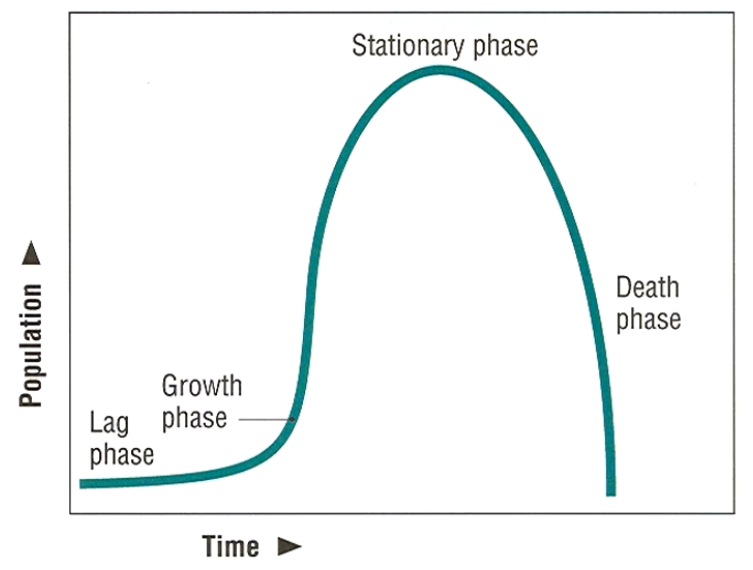
\includegraphics[width=0.50\textwidth]{curve}
\end{figure}
\begin{itemize}
    \item{\textbf{Lag phase} = \hl{delay} before population reproduce, \\ cells adjusting to new environment, cell growth enzyme synthesis}
    \item{\textbf{Log phase} = \hl{population increasing} at its \hl{fastest rate}; \\ binary fission doubles each division, exponential}
    \item{\textbf{Stationary phase} = \hl{mortality = natality}; \\ lack of space, shortage of nutrients, accumulation of toxic wastes}
    \item{\textbf{Death phase} = \hl{mortality $>$ natality}; nutrients run out, wastes accumulate, \\ \# of organisms decrease at a constant rate}
\end{itemize}

\pagebreak

\subsection{Growth Curve Types}
\begin{figure}[H]
    \centering
    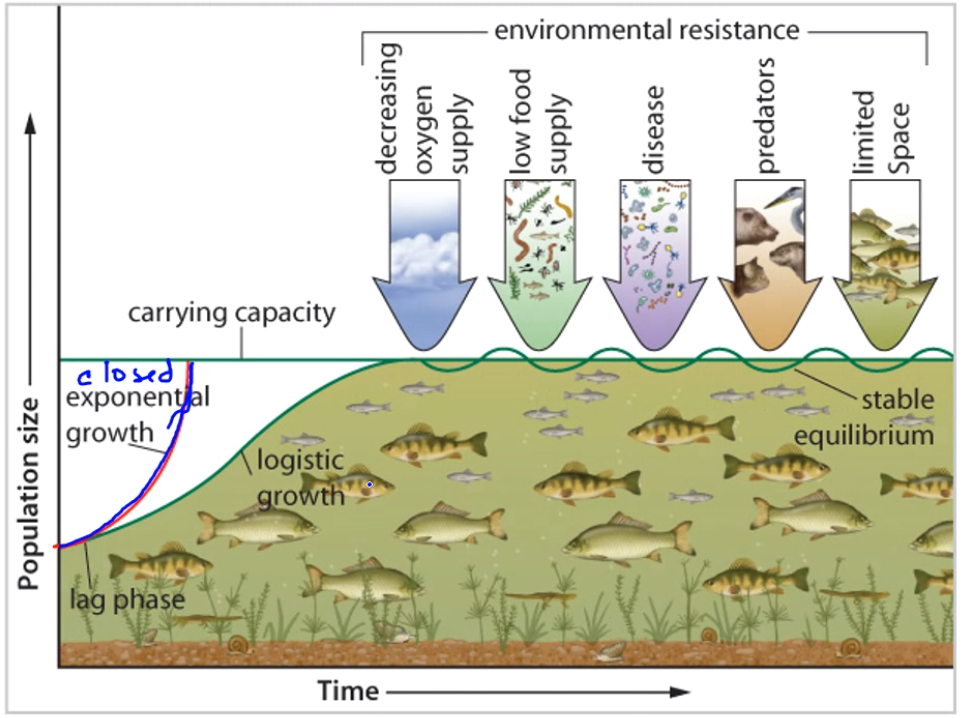
\includegraphics[width=0.7\textwidth]{curves}
\end{figure}
\begin{figure}[H]
    \centering
    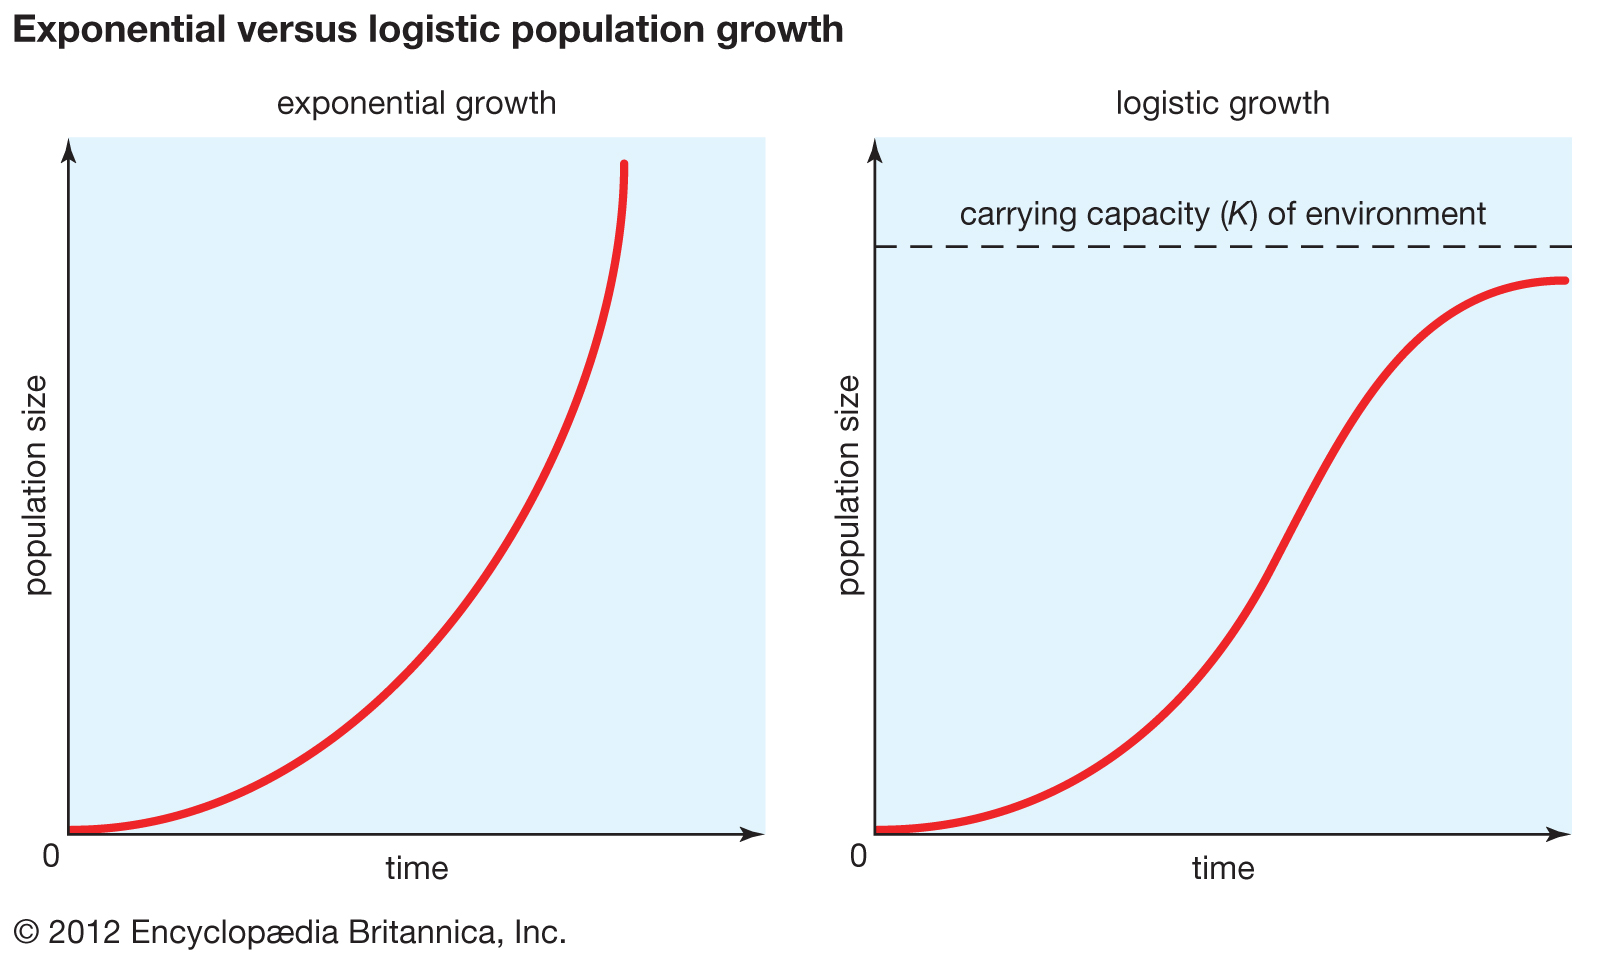
\includegraphics[width=0.75\textwidth]{scurve}
    \caption{J-shaped, closed system left; S-shaped, open system right}
\end{figure}
\subsubsection{J-shaped}
\begin{itemize}
    \item{Occurs in \hl{closed populations}}
    \item{\hl{Exponential growth}}
    \item{No carrying capacity}
\end{itemize}
\subsubsection{S-shaped}
\begin{itemize}
    \item{aka. Sigmoidal curve}
    \item{Occurs in \hl{open populations}, typical of an organism placed in a new environment}
\end{itemize}

\subsection{Biotic Potential ($R_{max}$)}
\begin{itemize}
    \item{Ability to reproduce at a \hl{typical rate} under \hl{ideal conditions}}
    \item{Ideal conditions --- \hl{not perfect}, some predators/disease/etc.}
    \item{
            Regulated by... (don't need to memorize)
            \begin{itemize}
                \item{Offspring = max \# of offspring per birth}
                \item{Capacity for survival = chance of offspring reaching reproductive age}
                \item{Procreation = \# times per year an organism reproduces}
                \item{Maturity = age at which reproduction begins}
            \end{itemize}
        }
\end{itemize}

\subsection{Environmental Resistance}
\begin{itemize}
    \item{All factors that \hl{limit population growth}}
    \item{\hl{Affect carrying capacity} of an environment}
    \item{Biotic and abiotic}
    \item{Continually changing}
    \item{For instance: predation, competition for space, disease}
    \item{\hl{Food is usually the most important \textbf{limiting factor}}}
\end{itemize}

\section{(22.3) Factors Affecting Population Change}
\begin{itemize}
    \item{\textbf{Minimum viable population} = smallest \# of individuals needed for a population to continue}
    \item{
            \textbf{Density dependent} = \hl{biotic affect biotic}; \\ factors brought on by population size may limit further growth and reduce population
            \begin{itemize}
                \item{Intraspecific competition: same species compete for resources}
            \end{itemize}
        }
    \item{\textbf{Density independent} = abiotic affect biotic; \\ abiotic factors that affect populations, regardless of its size}
    \item{\textbf{Law of the minimum} = the resource in shortest supply is the limiting factor}
\end{itemize}

\subsection{Strategies}
\begin{itemize}
    \item{
            \textbf{$K$ selected populations}
            \begin{itemize}
                \item{Environmental conditions are fairly stable, fluctuations are few}
                \item{Intense intraspecific competition}
                \item{Members are usually \hl{large, slow-growing, and require parental care}}
                \item{Usually S-shaped curves --- except humans, who are J-shaped}
                \item{Examples include elk, bears, coconut trees, \hl{humans}}
            \end{itemize}
        }
    \item{
            \textbf{$r$ selected populations}
            \begin{itemize}
                \item{Environmental condition flucuations can result in massive number of deaths}
                \item{Small, short life span, reproduce at a high rate}
                \item{J-shaped curves}
            \end{itemize}
        }
\end{itemize}

\section{(23) Population Interactions}
\subsection{Population Histograms}
\begin{figure}[H]
    \centering
    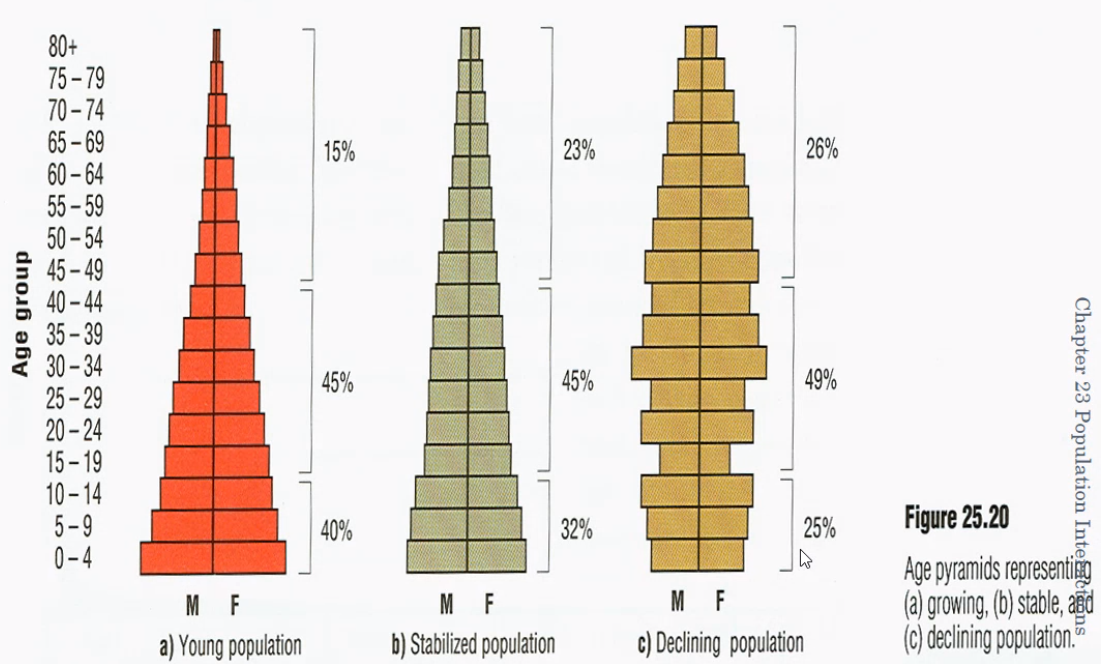
\includegraphics[width=\textwidth]{hist}
\end{figure}
\begin{itemize}
    \item{Don't need to know how to draw}
    \item{Wider = greater \# of individuals in population}
\end{itemize}

\subsubsection{Types}
\begin{itemize}
    \item{\textbf{Growing populations} = wide base, high \# of reproductive-capable animals}
    \item{\textbf{Stable populations} = young $>$ adult, growing very slowly, approaching zero growth}
    \item{\textbf{Population decline} = base narrower than middle}
\end{itemize}

\subsection{Human Population Growth}
\begin{itemize}
    \item{Industrial revolution = production of more food}
    \item{Transport systems = food distribution}
    \item{Reduction of infant mortality = water, health care}
\end{itemize}

\section{(23.1) Interactions within Communities}
\subsection{Interspecific Competition}
\begin{itemize}
    \item{\hl{Competition between different species}, restricts population growth}
    \item{\textbf{Interference competition} = aggression for same resource, e.g. stealing}
    \item{\textbf{Exploitative competition} = consumption of shared resources}
\end{itemize}

\subsection{Gause's Principle}
\begin{itemize}
    \item{If 2 populations of organisms occupy the \hl{same ecological niche}, one of the populations will be \hl{eliminated}}
    \item{
            Competition can be avoided by...
            \begin{itemize}
                \item{\textbf{Resource partitioning} = one species canges its behaviour; \\ i.e. use different resources, at different times, different places}
            \end{itemize}
        }
\end{itemize}

\end{document}
